% Kolmogorov-Arnold Networks in Recurrent Recommenders: complete report in one file.
% Generated by tools/flatten_report.py from report/main.tex; edit the sources, not this file.
% Compile with xelatex/tectonic or pdflatex (Overleaf). Optional files next to it:
%   figures (*.pdf from report/figures/) and upes_logo.png; missing ones show as placeholders.
% ---- preamble ----
\documentclass[12pt,a4paper]{report}

%  Packages 
\usepackage[a4paper, margin=1in]{geometry}
\usepackage{iftex}
\ifXeTeX
  \usepackage{fontspec}
  \setmainfont{texgyretermes}[Extension=.otf, UprightFont=*-regular, BoldFont=*-bold, ItalicFont=*-italic, BoldItalicFont=*-bolditalic]
\else
  \usepackage{times}
\fi
\usepackage{graphicx}
\usepackage{amsmath, amssymb}
\usepackage{booktabs}
\usepackage{array}
\usepackage{longtable}
\usepackage{hyperref}
\usepackage{url}
\usepackage{listings}
\usepackage{xcolor}
\usepackage{fancyhdr}
\usepackage{setspace}
\usepackage{titlesec}
\usepackage{caption}
\usepackage{subcaption}
\usepackage{float}
\usepackage{enumitem}
\usepackage{multirow}
\usepackage{algorithm}
\usepackage{algpseudocode}
\usepackage{tikz}
\usepackage{pgfplots}
\pgfplotsset{compat=1.18}
\usetikzlibrary{shapes.geometric, arrows, positioning, fit, backgrounds}

%  Fix paragraph indentation (no indent, small skip between paras) 
\usepackage{parskip}
\setlength{\parindent}{0pt}
\setlength{\parskip}{6pt plus 2pt minus 1pt}

%  Colors 
\definecolor{codegray}{RGB}{245, 245, 245}
\definecolor{codegreen}{RGB}{0, 128, 0}
\definecolor{codepurple}{RGB}{128, 0, 128}
\definecolor{codeblue}{RGB}{0, 82, 147}
\definecolor{winnergreen}{RGB}{220, 255, 220}
\definecolor{lightblue}{RGB}{235, 245, 255}

%  Hyperref setup 
\hypersetup{
    colorlinks=true,
    linkcolor=black,
    citecolor=black,
    urlcolor=black,
}

%  Code listing style 
\lstdefinestyle{pythonstyle}{
    backgroundcolor=\color{codegray},
    commentstyle=\color{codegreen},
    keywordstyle=\color{codeblue}\bfseries,
    stringstyle=\color{codepurple},
    basicstyle=\ttfamily\footnotesize,
    breaklines=true,
    frame=single,
    language=Python,
    showstringspaces=false,
    tabsize=4,
    captionpos=b
}

%  Page style 
\pagestyle{fancy}
\fancyhf{}
\fancyhead[L]{\small KAN in Recurrent Recommenders}
\fancyhead[R]{\small UPES, Dehradun}
\fancyfoot[C]{\thepage}
\renewcommand{\headrulewidth}{0.4pt}

%  Chapter/Section title format 
\titleformat{\chapter}[block]
  {\normalfont\large\bfseries\centering}
  {\thechapter.}{0.5em}{\large\bfseries\MakeUppercase}
\titlespacing*{\chapter}{0pt}{12pt}{12pt}

\titleformat{\section}[block]
  {\normalfont\normalsize\bfseries}
  {\thesection.}{0.5em}{}
\titlespacing*{\section}{0pt}{10pt}{6pt}

\titleformat{\subsection}[block]
  {\normalfont\normalsize\bfseries}
  {\thesubsection.}{0.5em}{}
\titlespacing*{\subsection}{0pt}{8pt}{4pt}

\titleformat{\subsubsection}[block]
  {\normalfont\normalsize\bfseries}
  {\thesubsubsection.}{0.5em}{}
\titlespacing*{\subsubsection}{0pt}{6pt}{4pt}

%  Line spacing 
\onehalfspacing

\setcounter{secnumdepth}{4}
\setcounter{tocdepth}{4}

% 

%  Tables and macros generated by the notebook 
\graphicspath{{figures/}{assets/}}
\newcommand{\generated}[1]{\IfFileExists{generated/#1}{}{\begin{center}\fbox{\parbox{0.8\textwidth}{\centering\small Table \texttt{generated/#1} is produced by \texttt{kan\_rec.ipynb}.}}\end{center}}}
\newcommand{\genfigure}[2]{\IfFileExists{figures/#1}{\includegraphics[#2]{figures/#1}}{\IfFileExists{#1}{\includegraphics[#2]{#1}}{\fbox{\parbox{0.8\textwidth}{\centering\small Figure \texttt{\detokenize{#1}} is produced by \texttt{kan\_rec.ipynb}.}}}}}
\newcommand{\kanLinearShare}{?}\newcommand{\kanMedianRtwo}{?}
\setlength{\emergencystretch}{2em}
\newcolumntype{L}[1]{>{\raggedright\arraybackslash}p{#1}}


\begin{document}

% 
% TITLE PAGE
% 
\begin{titlepage}
\centering
\vspace*{1cm}

{\Large \textbf{Kolmogorov-Arnold Networks in Recurrent Recommenders:\\[0.15cm]
Session-Based and Next-Basket Prediction}}\\[0.5cm]
{\large \textit{A}}\\[0.3cm]
{\large \textit{\textbf{Project Report}}}\\[0.2cm]
{\normalsize \textit{submitted in partial fulfillment of the}}\\
{\normalsize \textit{requirements for the award of the degree of}}\\[0.5cm]

{\Large \textbf{BACHELOR OF TECHNOLOGY}}\\[0.2cm]
{\large \textbf{in}}\\[0.2cm]
{\Large \textbf{COMPUTER SCIENCE \& ENGINEERING}}\\[0.8cm]

{\normalsize \textbf{by}}\\[0.5cm]

\begin{tabular}{ll}
\textbf{Name} & \textbf{Roll No.} \\
Saksham Agrawal & R2142231383 \\
Abhishek Yadav  & R2142231410 \\
Yash Dagar      & R2142231424 \\
\end{tabular}\\[0.8cm]

{\normalsize \textit{under the guidance of}}\\[0.3cm]
{\large \textbf{Dr. Amar Jindal}}\\[1.5cm]

\IfFileExists{assets/upes_logo.png}{\includegraphics[width=4cm]{assets/upes_logo.png}}{\IfFileExists{upes_logo.png}{\includegraphics[width=4cm]{upes_logo.png}}{\fbox{\parbox{4cm}{\centering\small UPES logo\\(upes\_logo.png)}}}}\\[0.5cm]

{\large \textbf{School of Computer Science}}\\
{\large \textbf{University of Petroleum \& Energy Studies}}\\
{\normalsize Bidholi, Via Prem Nagar, Dehradun, Uttarakhand}\\[0.4cm]
{\normalsize \textbf{January -- May, 2026}}

\end{titlepage}

\pagenumbering{roman}

% 
% CANDIDATE'S DECLARATION
% 
\chapter*{Candidate's Declaration}
\addcontentsline{toc}{chapter}{Candidate's Declaration}

I/We hereby certify that the project work entitled
\textbf{``Kolmogorov-Arnold Networks in Recurrent Recommenders: Session-Based and
Next-Basket Prediction''}
in partial fulfillment of the requirements for the award of the Degree of
\textbf{BACHELOR OF TECHNOLOGY} in
\textbf{COMPUTER SCIENCE AND ENGINEERING}
with specialization in \textbf{Artificial Intelligence and Machine Learning}
and submitted to the Department of Artificial Intelligence, School of Computer Science,
University of Petroleum \& Energy Studies, Dehradun, is an authentic record of
my/our work carried out during a period from \textbf{January, 2026} to
\textbf{May, 2026} under the supervision of
\textbf{Dr.\ Amar Jindal, Assistant Professor, Data Science Cluster, UPES}.

The matter presented in this project has not been submitted by me/us for the award
of any other degree of this or any other University.

\vspace{2cm}

\noindent
\begin{tabular}{p{4cm} p{4cm} p{4cm}}
\textbf{(Saksham Agrawal)} & \textbf{(Abhishek Yadav)} & \textbf{(Yash Dagar)} \\
\textbf{Roll No.\ R2142231383} & \textbf{Roll No.\ R2142231410} & \textbf{Roll No.\ R2142231424} \\
\end{tabular}

\vspace{1.5cm}
\noindent
This is to certify that the above statement made by the candidate is correct to the
best of my knowledge.

\vspace{1.5cm}

\noindent
Date: \underline{\hspace{3cm}} \hfill \textbf{Dr.\ Amar Jindal}\\
\hfill Project Guide

% 
% ACKNOWLEDGEMENT
% 
\chapter*{Acknowledgement}
\addcontentsline{toc}{chapter}{Acknowledgement}

We wish to express our deep gratitude to our guide \textbf{Dr.\ Amar Jindal},
for all advice, encouragement and constant support he has given us throughout our
project work. This work would not have been possible without his support and
valuable suggestions on integrating Kolmogorov-Arnold Networks into sequential
recommendation systems.

We sincerely thank our respected Head of Department, School of Computer
Science, UPES, for great support in doing our project, and for providing access
to the High-Performance Computing (HPC) cluster which was essential for training
our deep learning models.

We are also grateful to the Dean, SoCS, UPES for giving us the necessary facilities
to carry out our project work successfully. We also thank our Course
Coordinator and Activity Coordinator for providing timely support and information
during the completion of this project.

We acknowledge the use of the \textbf{YooChoose} dataset provided by the RecSys 2015
challenge organizers, the \textbf{Instacart} Market Basket Analysis dataset, and
the \textbf{dunnhumby} ``The Complete Journey'' dataset. We also thank the authors
of the official GRU4Rec implementation and of the next-basket GRU study by van
Maasakkers, Fok and Donkers for making their code public.

We would like to thank all our friends for their help and constructive criticism
during our project work. Finally, we have no words to express our sincere gratitude
to our parents who have shown us this world and for every support they have given us.

\vspace{1.5cm}

\noindent
\begin{tabular}{p{4cm} p{4cm} p{4cm}}
\textbf{Saksham Agrawal} & \textbf{Abhishek Yadav} & \textbf{Yash Dagar} \\
R2142231383 & R2142231410 & R2142231424 \\
\end{tabular}

% 
% ABSTRACT
% 
\chapter*{Abstract}
\addcontentsline{toc}{chapter}{Abstract}

% ---- chapters/abstract ----



% 
\tableofcontents
\listoffigures
\listoftables

\pagenumbering{arabic}

% ---- chapters/ch1_introduction ----
\chapter{Introduction}

\section{Background and Context}

Recommendation systems help users find relevant items in catalogues far too
large to browse, and they drive engagement on e-commerce sites, streaming
services and grocery platforms. Classical collaborative filtering builds
long-term user profiles from historical interactions. Many practical settings do
not provide such profiles: visitors are anonymous, sessions are short, or
privacy regulations such as GDPR limit tracking. Other settings provide long
histories but ask a different question, such as which products a customer will
buy on their next grocery trip.

This project studies two such sequential tasks:

\begin{itemize}
    \item \textbf{Session-based recommendation}: predict the next item clicked in
          an anonymous browsing session, using only the clicks so far in that
          session.
    \item \textbf{Next-basket recommendation}: predict the set of products in a
          customer's next shopping basket from the sequence of their previous
          baskets.
\end{itemize}

Both tasks are naturally modelled with recurrent neural networks (RNNs), and
the gated recurrent unit (GRU) is the standard building block in both: GRU4Rec
for sessions \cite{hidasi2016,hidasi2018} and the basket-GRU of van Maasakkers
et al.\ \cite{vanmaasakkers2023} for baskets.

\section{Session-Based Recommendation}

A session is a short sequence of user actions, here clicks on items, within a
limited time frame. Formally, given the items $S = (i_1, i_2, \ldots, i_t)$ of a
session so far, the model ranks all items by the probability that $i_{t+1}$ is
clicked next. Every position in a session is a prediction target. Sessions are
short (the median YooChoose session has two or three clicks), noisy and highly
variable, and the item catalogue contains tens of thousands of items with a long
popularity tail.

\section{Next-Basket Recommendation}

In next-basket recommendation each user $u$ has a history of baskets
$B^u_1, \ldots, B^u_{T}$, each a set of items, and the model ranks all items for
the unseen basket $B^u_{T+1}$. Next-basket data differ from session data in two
ways. Histories are long (tens of baskets per customer), and a large share of
each next basket consists of items the customer has bought before (\emph{repeat}
items). Recent work showed that this repeat behaviour dominates the achievable
accuracy, and that simple personal-frequency baselines are very hard to beat
\cite{li2023}.

\section{Kolmogorov-Arnold Networks}

Kolmogorov-Arnold Networks (KANs) \cite{liu2025kan} are motivated by the
Kolmogorov-Arnold representation theorem, which states that any continuous
function $f:[0,1]^n \to \mathbb{R}$ can be written as
\begin{equation}
f(x_1, \ldots, x_n) = \sum_{q=0}^{2n} \Phi_q \left( \sum_{p=1}^{n} \phi_{q,p}(x_p) \right),
\end{equation}
where $\phi_{q,p}$ and $\Phi_q$ are continuous univariate functions. A KAN layer
mapping $d_{in}$ inputs to $d_{out}$ outputs places a learnable univariate
function on every edge,
\begin{equation}
y_o = \sum_{i=1}^{d_{in}} \phi_{o,i}(x_i), \qquad o = 1, \ldots, d_{out},
\end{equation}
so a layer contains $d_{in} \times d_{out}$ learnable functions, each usually
parameterised as a linear combination of basis functions such as B-splines. An
MLP layer instead applies one fixed non-linearity after a linear map.

The properties usually claimed for KANs are better accuracy per parameter on
smooth function-fitting problems and interpretability, because each learned edge
function can be plotted. Later studies qualify these claims: when parameters and
FLOPs are matched, KANs outperform MLPs mainly on symbolic formula fitting
\cite{yu2024}, and they are considerably slower to train \cite{hou2025}. Whether
KAN layers help recommendation models therefore has to be tested against
carefully controlled baselines.

\section{Motivation: Findings of the First Draft}

A first version of this project compared a 2-layer GRU, an ungated ``pure
recurrent KAN'' and a GRU+KAN hybrid on a random 50,000-session sample of
YooChoose. The KAN models lost on every metric and trained up to 10.8 times more
slowly. A review of that work found that its protocol leaked test information
into training, used the test set for model selection, and that its B-spline
implementation produced piecewise-constant step functions rather than cubic
splines (Appendix~\ref{app:errata}). Those numbers are therefore not reliable
evidence either for or against KANs, and this report replaces them.

\section{Problem Statement}

Determine whether, and where, KAN layers improve GRU-based recommenders, under
a protocol that permits a fair conclusion:

\begin{itemize}
    \item standard, leakage-free data splits that make results comparable with
          published work;
    \item correct, independently verified implementations of both the baselines
          and the KAN layers;
    \item controls that separate the effect of the KAN from the effect of simply
          adding parameters;
    \item evaluation on both session-based and next-basket data.
\end{itemize}

\section{Project Objectives}

\begin{enumerate}
    \item Correct the methodological and reporting errors of the first draft.
    \item Implement a KAN layer with four basis families (B-spline, Gaussian RBF,
          Chebyshev, rational) and verify it with unit tests.
    \item Extend the official GRU4Rec implementation with KAN layers in three
          placements: on the final hidden state, on the input embedding, and
          inside the GRU cell, each paired with a parameter-matched MLP control.
    \item Apply the same placements to the basket-GRU on the Instacart and
          Dunnhumby next-basket datasets, following the preprocessing of
          \cite{vanmaasakkers2023}.
    \item Compare against strong non-neural baselines (item-kNN, personal top
          frequency, TIFU-KNN) and report accuracy, cost, statistical
          significance and the interpretability of the learned functions.
    \item Propose KAN-NBR, a small additive KAN over interpretable repeat-purchase
          features, and test whether its learned functions add accuracy or
          insight over logistic regression and a parameter-matched MLP.
\end{enumerate}

\section{Report Organisation}

Chapter~\ref{ch:literature} reviews related work on session-based and
next-basket recommendation and on KANs. Chapter~\ref{ch:data} describes the
datasets and preprocessing protocols. Chapter~\ref{ch:models} presents the KAN
layer and the model variants. Chapter~\ref{ch:setup} covers the experimental
setup, and Chapter~\ref{ch:results} the results. Chapter~\ref{ch:conclusion}
concludes. The appendices contain the core code and the errata for the first
draft.

% ---- chapters/ch2_literature ----
\chapter{Literature Review}
\label{ch:literature}

\section{Session-Based Recommendation}

Early session-based recommenders relied on item-to-item similarity: the item-kNN
approach recommends the items that most often co-occur in sessions with the
current item. It remains a strong baseline.

\textbf{Hidasi et al.\ (2016)} \cite{hidasi2016} introduced GRU4Rec, the first
RNN for session-based recommendation. Its central engineering contribution is
\emph{session-parallel mini-batches}: each mini-batch slot holds one session and
advances one click per step; when a session ends, a new session takes its slot
and the slot's hidden state is reset. On YooChoose, GRU4Rec clearly outperformed
item-kNN.

\textbf{Hidasi and Karatzoglou (2018)} \cite{hidasi2018} improved GRU4Rec with
additional negative samples shared across the mini-batch and drawn in proportion
to popularity$^\alpha$, and with the BPR-max and TOP1-max ranking losses, raising
Recall@20 on the full YooChoose data from 0.585 to 0.721. This improved version
is the one used in this project.

\textbf{Hidasi and Czapp (2023)} \cite{hidasi2023} examined six third-party
implementations of GRU4Rec used in comparative studies and found that they
scored 30--99\% below the official implementation, because of incorrect loss
functions, wrong hidden-state handling, missing negative sampling, or broken
dropout. Many papers that report GRU4Rec as a weak baseline used such
implementations. For this reason all session-based models in this project are
built on the official PyTorch code.

\textbf{Li et al.\ (2017)} \cite{li2017} proposed NARM, which adds an attention
mechanism over the GRU hidden states to capture the user's main purpose in the
session. \textbf{Liu et al.\ (2018)} \cite{liu2018} proposed STAMP, an
attention-based model of short-term interest. \textbf{Wu et al.\ (2019)}
\cite{wu2019} modelled sessions as graphs with SR-GNN. These papers established
the standard yoochoose1/64 and yoochoose1/4 benchmarks used in
Chapter~\ref{ch:results}.

\textbf{Kang and McAuley (2018)} \cite{kang2018} proposed SASRec, a
self-attentive sequential recommender, and \textbf{Sun et al.\ (2019)}
\cite{sun2019} the bidirectional BERT4Rec. Transformer-based models capture
long-range dependencies but are larger and more expensive than GRU4Rec.

\section{Next-Basket Recommendation}

\textbf{Rendle et al.\ (2010)} \cite{rendle2010} introduced FPMC, which combines
matrix factorisation with a personalised Markov chain over consecutive baskets.
\textbf{Yu et al.\ (2016)} \cite{yu2016} proposed DREAM, the first RNN for
next-basket recommendation, which pools the item embeddings of each basket and
feeds the pooled vectors to an RNN.

\textbf{Guidotti et al.\ (2019)} \cite{guidotti2019} proposed TARS, which mines
temporal annotated recurring sequences from each customer's own history and
predicts the next basket from them; it is interpretable by construction. Its
implementation, \texttt{tbp-next-basket}, also provides an evaluation suite of
set-based precision, recall, F-scores and hit rate.

\textbf{Hu and He (2019)} \cite{hu2019} proposed Sets2Sets, an encoder-decoder
with an explicit repeat component. \textbf{Hu et al.\ (2020)} \cite{hu2020}
showed with TIFU-KNN that a simple method based on time-decayed personal item
frequencies, combined with the frequencies of nearest-neighbour users,
outperforms most neural models. \textbf{Ariannezhad et al.\ (2022)}
\cite{ariannezhad2022} proposed ReCANet, a model dedicated to repeat
consumption.

\textbf{Li et al.\ (2023)} \cite{li2023} re-evaluated next-basket methods and
found that repeat items account for most of the correct predictions on Instacart
and Dunnhumby, that personal-frequency baselines are very strong, and that
several neural models perform close to global popularity. They recommend
reporting repeat and explore performance separately, which this project does.

\textbf{Van Maasakkers, Fok and Donkers (2023)} \cite{vanmaasakkers2023} applied
a GRU directly to multi-hot basket vectors, with a sigmoid output for every
product, on Instacart and Dunnhumby (The Complete Journey). With large hidden
layers (750 and 1500 units) the GRU outperformed personal frequency and TARS on
most metrics. Their preprocessing and evaluation protocol is followed here, and
their basket-GRU is the next-basket baseline that KAN layers are added to.

\section{Kolmogorov-Arnold Networks}

\textbf{Liu et al.\ (2025)} \cite{liu2025kan} introduced KANs, which place a
learnable univariate function, parameterised by B-splines, on every edge. On
small scientific and function-fitting tasks KANs reached a given accuracy with
fewer parameters than MLPs and allowed learned functions to be inspected and
even replaced by symbolic formulas. The authors identified slow training as the
main limitation.

Two later studies qualify these results. \textbf{Yu, Yu and Wang (2024)}
\cite{yu2024} compared KANs and MLPs with matched parameters and FLOPs across
machine learning, computer vision, NLP, audio and symbolic formula
representation; KANs were better only on symbolic formulas, and an MLP given
B-spline activations matched or exceeded KAN elsewhere.
\textbf{Hou et al.\ (2025)} \cite{hou2025} critically assessed the claims made
for KANs and reported that they are substantially slower to train than MLPs and
rarely more accurate outside symbolic regression. Both studies motivate the
parameter-matched MLP controls used in this project.

Several cheaper bases have been proposed. \textbf{FastKAN} \cite{li2024fastkan}
replaces B-splines with Gaussian radial basis functions and shows that a KAN
with such a basis is a radial basis function network. Chebyshev-polynomial KANs
\cite{ss2024cheby} use orthogonal polynomials on tanh-bounded inputs, and
ReLU-KAN \cite{relukan} builds the basis from ReLU products. The
\textbf{Kolmogorov-Arnold Transformer} \cite{yang2025kat} introduced group-rational
KAN (GR-KAN) layers, in which rational functions are shared within groups of
input channels, and used them as drop-in replacements for the MLP blocks of
vision transformers.

\section{KANs for Sequential and Temporal Data}

\textbf{Xu, Chen and Wang (2024)} \cite{xu2024tskan} applied KANs to time-series
forecasting and argued that the learned univariate functions make the models
interpretable. \textbf{Genet and Inzirillo (2024)} \cite{genet2024} proposed TKAN,
a recurrent cell that keeps the LSTM's sigmoid gates and memory cell and uses KAN
layers only inside the recurrent transformation. TKAN shows that KANs can be
placed inside a recurrent cell without giving up gating; the KAN-GRU cell of
Chapter~\ref{ch:models} follows the same principle.

\section{KANs in Recommender Systems}

\textbf{CF-KAN} \cite{park2024cfkan} replaces the MLP of an autoencoder-based
collaborative filtering model with a KAN and reports higher Recall@20 than strong
collaborative filtering baselines on MovieLens-1M, Yelp and Anime, together with
more robustness to catastrophic forgetting. It is, to our knowledge, the only KAN
recommender that compares against an MLP version of the same model with the same
number of parameters, and it is not yet peer-reviewed. \textbf{FourierKAN-GCF}
\cite{xu2024fkgcf} replaces the feature transformation in graph collaborative
filtering with a Fourier-basis KAN. \textbf{KANRec} \cite{xu2026kanrec} uses KAN
layers to fuse global and local interests in sequential recommendation.

\section{Summary of Related Work}


\begin{table}[H]
\centering
\caption{Summary of the main related work.}
\label{tab:related}
\small
\begin{tabular}{L{3.2cm} L{1.3cm} L{2.7cm} L{2.5cm} L{3.9cm}}
\toprule
\textbf{Work} & \textbf{Year} & \textbf{Model} & \textbf{Data} & \textbf{Relevance / limitation} \\
\midrule
Hidasi et al.\ \cite{hidasi2016,hidasi2018} & 2016/18 & GRU4Rec & YooChoose & Strong session baseline; reimplementations often flawed \cite{hidasi2023} \\
Li et al.\ \cite{li2017} & 2017 & NARM (GRU + attention) & YooChoose, Diginetica & Standard benchmark; black-box attention \\
Wu et al.\ \cite{wu2019} & 2019 & SR-GNN & YooChoose, Diginetica & Standard yoochoose1/64 table \\
Yu et al.\ \cite{yu2016} & 2016 & DREAM (RNN) & Ta-Feng, T-Mall & Close to popularity in later re-evaluations \cite{li2023} \\
Guidotti et al.\ \cite{guidotti2019} & 2019 & TARS & Coop, Ta-Feng & Interpretable; per-customer, slow \\
Hu et al.\ \cite{hu2020} & 2020 & TIFU-KNN & Instacart, Dunnhumby & Simple frequency model beats neural models \\
Li et al.\ \cite{li2023} & 2023 & Re-evaluation & Instacart, Dunnhumby, Ta-Feng & Repeat items dominate accuracy \\
van Maasakkers et al.\ \cite{vanmaasakkers2023} & 2023 & Basket-GRU & Instacart, Dunnhumby & Our basket baseline and protocol \\
Liu et al.\ \cite{liu2025kan} & 2025 & KAN & Function fitting, science & Slow training \\
Yu et al.\ \cite{yu2024} & 2024 & KAN vs MLP & Many domains & KAN rarely wins when matched \\
Genet and Inzirillo \cite{genet2024} & 2024 & TKAN & Time series & KAN inside a gated cell \\
Park et al.\ \cite{park2024cfkan} & 2024 & CF-KAN & ML-1M, Yelp, Anime & KAN in collaborative filtering \\
Xu et al.\ \cite{xu2026kanrec} & 2026 & KANRec & Sequential rec. & KAN interest fusion \\
\bottomrule
\end{tabular}
\end{table}

\section{Research Gap}

KAN layers have been applied to collaborative filtering, graph recommendation and
attention-based sequential recommendation, and KAN components have been placed
inside gated recurrent cells for time series. We found no work that places KAN
layers inside GRU4Rec, the most widely used RNN for session-based recommendation,
or that applies KANs to next-basket recommendation, and among the KAN
recommenders we found, only CF-KAN controls for model size with a
parameter-matched MLP. The first draft of this
project also showed how easily such comparisons go wrong: without a standard
protocol, a verified implementation and a capacity-matched control, neither a
gain nor a loss can be attributed to the KAN. This project therefore asks a
narrower question than ``are KANs better?'': \emph{where in a GRU-based
recommender, if anywhere, does a KAN layer help, compared with an MLP of the same
size, on standard session and basket benchmarks?}

% ---- chapters/ch3_data ----
\chapter{Datasets and Preprocessing}
\label{ch:data}

Three public datasets are used: YooChoose for session-based recommendation, and
Instacart and Dunnhumby for next-basket recommendation. All three are downloaded
from Kaggle by the notebook. All preprocessing follows published protocols so
that the results can be compared with prior work, and every statistic in this
chapter is computed and exported by the notebook.

\section{YooChoose (Session-Based)}

YooChoose is the click log of the ACM RecSys Challenge 2015 \cite{benshimon2015},
collected from a European e-commerce site over six months in 2014. Each row
contains a session ID, a timestamp, an item ID and a category; the click file has
33,003,944 rows.

\subsection{Protocol}

The preprocessing follows GRU4Rec \cite{hidasi2016} and the yoochoose1/64 split
used by NARM, STAMP and SR-GNN \cite{li2017,liu2018,wu2019}:

\begin{enumerate}
    \item Remove sessions with a single click, then items that occur in fewer than
          5 sessions, then sessions that have become shorter than 2 clicks.
    \item \textbf{Test set}: all sessions that end during the last day of the log.
    \item \textbf{Training data}: the most recent 1/64 of the remaining sessions
          (ordered by start time). This is the common yoochoose1/64 setting; the
          UPES profile also runs yoochoose1/4.
    \item \textbf{Validation set}: the sessions of the last day of that training
          data are held out for early stopping and model selection.
    \item Validation and test keep only items that occur in the final training
          data; sessions shorter than 2 clicks after this filter are removed.
\end{enumerate}

Every click after the first in a validation or test session is a prediction
target, so a session of length $n$ contributes $n-1$ predictions. Because the
split is by session and by time, no session contributes to more than one split.
The notebook asserts this, and that every training session ends before the
validation window and every validation session before the test window. This
removes the leakage of the first draft, where prefixes of the same session were
shuffled into both training and test sets.

\begin{center}\fbox{\parbox{0.8\textwidth}{\centering\small Table \texttt{generated/dataset\_yoochoose.tex} is produced by \texttt{kan\_rec.ipynb}.}}\end{center}

The resulting split closely matches the one reported by SR-GNN for
yoochoose1/64 (55,898 test predictions and 16,766 items in \cite{wu2019}).

\begin{figure}[H]
\centering
\genfigure{eda.pdf}{width=\textwidth}
\caption{Left: clicks per session in the raw YooChoose log (log scale). Centre:
item popularity by rank (log-log), showing the long tail. Right: number of
baskets per user in the two next-basket datasets.}
\label{fig:eda}
\end{figure}

\section{Instacart (Next-Basket)}

The Instacart Market Basket Analysis data contain over three million grocery
orders from 206,209 users, with 49,688 products in 134 aisles. Each user has
between 4 and 100 orders. Kaggle's \texttt{eval\_set} column marks every user's
final order as either \emph{train} (products given) or \emph{test} (products
hidden for the competition).

\subsection{Protocol}

Following van Maasakkers et al.\ \cite{vanmaasakkers2023}:

\begin{enumerate}
    \item Drop the hidden Kaggle \emph{test} orders; each user's last remaining
          order is the target basket and all earlier orders are the history.
    \item \textbf{Product clustering.} Rare products (fewer than 500 purchases in
          the training history) are merged within their aisle. The authors'
          R script merges greedily by cosine similarity of the products' purchase
          vectors; we re-implemented it in Python, merging the rarest cluster with
          its most similar rare cluster in the same aisle until every cluster
          reaches 500 purchases or the aisle has no rare products left. Frequent
          products keep their own index. Products that appear only in target
          baskets are removed.
    \item Users are split at random into equal validation and test groups. The
          target basket of a validation user is used for early stopping; the
          target basket of a test user for the final evaluation. The histories of
          all users are used for training.
\end{enumerate}

Our clustering yields 12,058 product groups, against 9,407 in the original
paper, because our implementation only merges rare products with each other,
whereas the original evidently also merged more aggressively. On the Mac profile a random 10\% of users is used, as in the
NBR re-evaluation study \cite{li2023}; the GPU profiles use all users.

\section{Dunnhumby: The Complete Journey (Next-Basket)}

The Complete Journey contains two years of transactions of 2,500 households at a
retailer: 2,595,732 transaction rows over 92,339 products, with the household,
basket, day and time of each purchase.

\subsection{Protocol}

Following van Maasakkers et al.\ \cite{vanmaasakkers2023}:

\begin{enumerate}
    \item Keep products bought at least 50 times and households with at least 3
          baskets.
    \item Order each household's baskets by day and transaction time and keep the
          \emph{100 most recent} baskets. (The published script keeps the first
          100 baskets, which discards the most recent history of 37\% of the
          households; we keep the most recent ones.)
    \item The last basket of each household is the target; households are split
          at random into equal validation and test groups.
\end{enumerate}

After preprocessing the data contain 2,478 households, 10,370 products, 163,937
baskets and 66.16 baskets per household. These figures are identical to those
reported by van Maasakkers et al.

Note that several next-basket benchmarks, including TIFU-KNN \cite{hu2020} and
the NBR re-evaluation \cite{li2023}, use a different Dunnhumby dataset (``Let's
Get Sort-of-Real''), so their Dunnhumby results are not comparable with ours.

\begin{center}\fbox{\parbox{0.8\textwidth}{\centering\small Table \texttt{generated/dataset\_baskets.tex} is produced by \texttt{kan\_rec.ipynb}.}}\end{center}

\section{Repeat Behaviour}

The ``Repeat ratio'' row of Table~\ref{tab:basket_stats} gives the average share
of a target basket that the customer had bought before. It is about 0.60 on
Instacart and 0.53 on Dunnhumby, in line with the 60\% and 51\% reported by van
Maasakkers et al. Repeat items are much easier to predict than new ones
\cite{li2023}, which is why the results in Chapter~\ref{ch:results} are also
reported separately for repeat and explore items.

% ---- chapters/ch4_models ----
\chapter{Model Architectures}
\label{ch:models}

This chapter describes the KAN layer, the two recurrent baselines, and the
places where KAN layers are inserted into them. Every equation corresponds
directly to the code in \texttt{kanrec/kan.py}, \texttt{kanrec/session.py} and
\texttt{kanrec/basket.py}.

\section{The KAN Layer}

\subsection{Definition}

A KAN layer with $d_{in}$ inputs and $d_{out}$ outputs computes
\begin{equation}
y_o = \sum_{i=1}^{d_{in}} \Big( w^{b}_{o,i}\, \mathrm{silu}(x_i) + \sum_{k=1}^{K} c_{o,i,k}\, B_k(x_i) \Big) + b_o,
\qquad o = 1, \ldots, d_{out},
\label{eq:kan}
\end{equation}
where $B_1, \ldots, B_K$ are fixed basis functions, $c_{o,i,k}$ are learnable
coefficients and $w^b_{o,i}$, $b_o$ form a linear ``base'' path on
$\mathrm{silu}(x)$, as in the efficient implementations of the original KAN
\cite{liu2025kan}. Each of the $d_{in} d_{out}$ edges therefore carries its own
learnable univariate function
\begin{equation}
\phi_{o,i}(x) = w^b_{o,i}\,\mathrm{silu}(x) + \sum_{k} c_{o,i,k} B_k(x),
\end{equation}
which can be plotted for interpretation (Section~\ref{sec:interp}). The layer
has $d_{in} d_{out} (K + 1) + d_{out}$ parameters, compared with
$d_{in} d_{out} + d_{out}$ for a linear layer.

\subsection{Basis Families}

Four basis families are implemented:

\begin{itemize}
    \item \textbf{B-spline} (cubic, $p = 3$, grid size $G$). With uniform knots
          $t_j = t_0 + jh$ on an extended grid that adds $p$ knots beyond each end
          of the range, the bases follow the Cox-de~Boor recursion
          \begin{align}
          B^{(0)}_j(x) &= \mathbb{1}[t_j \le x < t_{j+1}], \\
          B^{(q)}_j(x) &= \frac{x - t_j}{t_{j+q} - t_j}\, B^{(q-1)}_j(x)
                       + \frac{t_{j+q+1} - x}{t_{j+q+1} - t_{j+1}}\, B^{(q-1)}_{j+1}(x),
          \end{align}
          giving $K = G + p$ bases that sum to one everywhere inside the grid.
          The unit tests check this partition of unity and compare the bases with
          the closed-form uniform cubic B-spline.
    \item \textbf{Gaussian RBF} (FastKAN \cite{li2024fastkan}):
          $B_k(x) = \exp\!\big(-((x - \mu_k)/h)^2\big)$ with $K = G$ centres
          $\mu_k$ evenly spaced over the grid range and $h$ their spacing.
    \item \textbf{Chebyshev} \cite{ss2024cheby}: $B_k(x) = T_{k-1}(\tanh x)$,
          $k = 1, \ldots, G+1$, where $T_n$ are Chebyshev polynomials,
          computed with $T_0 = 1$, $T_1(u) = u$, $T_{n}(u) = 2uT_{n-1}(u) - T_{n-2}(u)$.
    \item \textbf{Group rational} (GR-KAN \cite{yang2025kat}): the inputs are split
          into 8 groups; within a group every input passes through the same
          learnable rational function
          \begin{equation}
          R(x) = \frac{\sum_{m=0}^{5} a_m x^m}{1 + \big|\sum_{n=1}^{4} b_n x^n\big|},
          \end{equation}
          followed by a linear layer. Functions are shared per group rather than
          per edge, so this variant is much smaller.
\end{itemize}

The B-spline and RBF grids span $[-2, 2]$, which covers inputs normalised by
LayerNorm; the default grid size is $G = 8$.

\subsection{Residual Block and MLP Control}

KAN layers are inserted as residual blocks,
\begin{equation}
\mathrm{Block}(\mathbf{h}) = \mathbf{h} + f\big(\mathrm{LayerNorm}(\mathbf{h})\big),
\label{eq:block}
\end{equation}
with $f$ a $d \to d$ KAN layer. The output layer of $f$ is initialised to zero,
so every block starts as the identity and every variant starts as exactly its
baseline model; the LayerNorm keeps the inputs inside the basis grid. For each KAN block, a \textbf{control block} uses the same
wrapper with $f(\mathbf{x}) = W_2\, \mathrm{silu}(W_1 \mathbf{x} + b_1) + b_2$, a
two-layer MLP whose hidden width is chosen so that it has the same number of
parameters as the KAN (within 2\%). A KAN block that beats the baseline but not
its control has shown only that the extra capacity helps.

\section{Session Model: GRU4Rec}

GRU4Rec \cite{hidasi2016,hidasi2018} with the official settings for YooChoose
uses one GRU layer of 480 units and \emph{constrained embeddings}: the item
embedding matrix $E$ is shared between input and output. For an input item $i_t$,
\begin{align}
\mathbf{x}_t &= E_{i_t}, \\
\mathbf{r}_t &= \sigma(W_{ir}\mathbf{x}_t + b_{ir} + W_{hr}\mathbf{h}_{t-1} + b_{hr}), \\
\mathbf{z}_t &= \sigma(W_{iz}\mathbf{x}_t + b_{iz} + W_{hz}\mathbf{h}_{t-1} + b_{hz}), \\
\mathbf{n}_t &= \tanh\big(W_{in}\mathbf{x}_t + b_{in} + \mathbf{r}_t \odot (W_{hn}\mathbf{h}_{t-1} + b_{hn})\big), \\
\mathbf{h}_t &= (1 - \mathbf{z}_t) \odot \mathbf{n}_t + \mathbf{z}_t \odot \mathbf{h}_{t-1},
\end{align}
and the score of item $j$ is $s_j = E_j^\top \mathbf{h}_t + \beta_j$.
(These are the PyTorch \texttt{GRUCell} equations; the first draft's candidate
equation was incorrect.) Training uses session-parallel mini-batches of 48
sessions, 2048 additional negative items shared across the mini-batch and
sampled in proportion to popularity$^{0.2}$, a softmax cross-entropy loss over
the targets and samples with a $\log Q$ popularity correction, dropout 0.2 on the
hidden state, and Adagrad with learning rate 0.07.

\section{KAN Placements in GRU4Rec}

\begin{figure}[H]
\centering
\resizebox{\textwidth}{!}{%
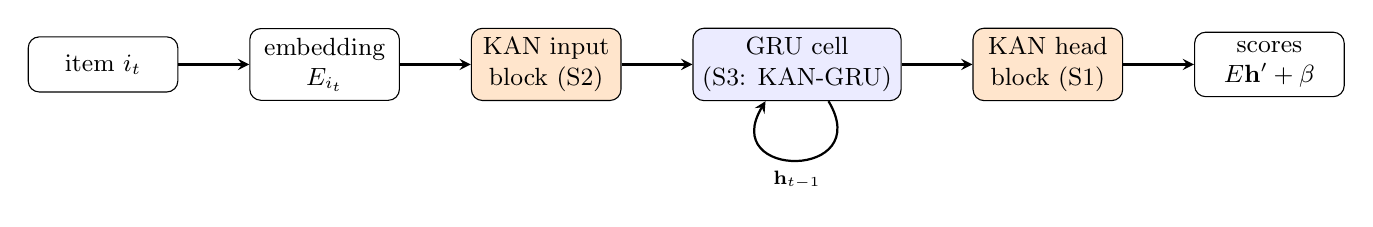
\begin{tikzpicture}[
  node distance=0.55cm and 0.9cm,
  box/.style={draw, rounded corners, minimum height=0.7cm, minimum width=1.9cm, align=center, font=\small},
  kan/.style={box, fill=orange!20},
  arr/.style={-{stealth}, thick}]
\node[box] (item) {item $i_t$};
\node[box, right=of item] (emb) {embedding\\$E_{i_t}$};
\node[kan, right=of emb] (kin) {KAN input\\block (S2)};
\node[box, right=of kin, fill=blue!8] (gru) {GRU cell\\(S3: KAN-GRU)};
\node[kan, right=of gru] (kout) {KAN head\\block (S1)};
\node[box, right=of kout] (score) {scores\\$E\mathbf{h}' + \beta$};
\draw[arr] (item) -- (emb);
\draw[arr] (emb) -- (kin);
\draw[arr] (kin) -- (gru);
\draw[arr] (gru) -- (kout);
\draw[arr] (kout) -- (score);
\draw[arr] ([xshift=0.4cm]gru.south) .. controls +(0.6,-1.0) and +(-0.6,-1.0) .. node[below, font=\scriptsize]{$\mathbf{h}_{t-1}$} ([xshift=-0.4cm]gru.south);
\end{tikzpicture}}
\caption{KAN placements in GRU4Rec. Orange blocks are optional residual KAN (or
MLP control) blocks; the GRU cell can be replaced by the KAN-GRU cell.}
\label{fig:placements}
\end{figure}

\begin{itemize}
    \item \textbf{S1, KAN head}: $\mathbf{h}'_t = \mathrm{Block}(\mathbf{h}_t)$
          before scoring. The block refines the session representation; scoring
          stays a dot product, so sampled negatives and constrained embeddings
          work unchanged. (A KAN on the item-scoring layer itself would need
          $480 \times 17{,}000 \times K$ coefficients.)
    \item \textbf{S2, KAN input}: $\mathbf{x}'_t = \mathrm{Block}(E_{i_t})$, a
          non-linear transformation of the item embedding before the GRU.
    \item \textbf{S1+S2}: both blocks.
    \item \textbf{S3, KAN-GRU cell}: the update and reset gates keep their linear
          + sigmoid form, as in TKAN \cite{genet2024}, and only the candidate
          state is computed by a KAN:
          \begin{equation}
          \mathbf{n}_t = \tanh\big(\mathrm{KAN}([\mathbf{x}_t;\ \mathbf{r}_t \odot \mathbf{h}_{t-1}])\big).
          \end{equation}
    \item \textbf{Draft models}, for continuity with the first draft:
          \emph{Draft Pure KAN} replaces the GRU with the ungated cell
          $\mathbf{h}_t = \tanh(\mathrm{LayerNorm}(\mathrm{KAN}([\mathbf{x}_t;\mathbf{h}_{t-1}])))$
          with a correct cubic B-spline basis, and \emph{Draft Hybrid} stacks that
          cell on top of a GRU layer.
\end{itemize}

S1 and S2 are paired with parameter-matched MLP controls (\emph{+MLP head},
\emph{+MLP input}), and S3 with the \emph{MLP-GRU cell}, whose candidate state
$\tanh(\mathrm{MLP}([\mathbf{x}_t; \mathbf{r}_t \odot \mathbf{h}_{t-1}]))$ uses an MLP with
the same number of parameters as the KAN. Draft Hybrid has two recurrent layers,
so it is compared with a two-layer GRU4Rec (same depth) and with \emph{Draft
Hybrid (MLP)}, in which the KAN of the ungated cell is replaced by a
parameter-matched MLP. Unless stated otherwise the KAN layers use the RBF basis
with $G=8$; the other bases are compared in an ablation.

\section{Next-Basket Model: Basket-GRU}

The basket-GRU of van Maasakkers et al.\ \cite{vanmaasakkers2023} reads the
multi-hot vector $\mathbf{m}_t \in \{0,1\}^N$ of basket $t$ and outputs a purchase
probability for every one of the $N$ items:
\begin{align}
\mathbf{x}_t &= W_{in}\mathbf{m}_t, \\
\mathbf{h}_t &= \mathrm{GRU}(\mathbf{x}_t, \mathbf{h}_{t-1}), \\
\hat{\mathbf{y}}_{t+1} &= \sigma(W_{out}\mathbf{h}_t + \mathbf{b}),
\end{align}
trained with binary cross-entropy against $\mathbf{m}_{t+1}$, averaged over all
items and over every step of every training history. The output bias $b_j$ is
initialised to the log-odds of item $j$'s share of training baskets, so that
training starts from the popularity predictor; without this, the biases need
thousands of updates to move from probability 0.5 towards the true base rates
of roughly $10^{-3}$, and short training runs stay at chance level. $W_{in}\mathbf{m}_t$ is
implemented as a sum-pooled embedding bag. Sequences of different lengths are
padded on the right and the representation of a user is read at their true last
basket (not at the last padded position, the error suspected in the first draft).
The KAN placements mirror those of GRU4Rec: \emph{+KAN head} applies
Equation~\eqref{eq:block} to $\mathbf{h}_t$, \emph{+KAN input} to $\mathbf{x}_t$,
and \emph{KAN-GRU cell} uses the cell of S3, each with its MLP control. As before, no KAN is applied on the
$N$-dimensional side.

\section{KAN-NBR: An Interpretable Repeat-Aware Model}
\label{sec:kannbr}

Because repeat purchases account for most of the achievable next-basket
accuracy \cite{li2023}, we also test a KAN where its interpretability can matter:
on a few meaningful scalar features rather than on hundreds of hidden units.
For user $u$ and candidate item $j$, where the candidates are the items $u$ has
bought before plus the 100 most popular items, KAN-NBR computes seven features
from the history $B^u_1, \ldots, B^u_n$:

\begin{enumerate}
    \item $\log(1 + \text{baskets since the last purchase of } j)$;
    \item $\log(1 + c_{uj})$, where $c_{uj}$ is the number of baskets containing $j$;
    \item the purchase share $c_{uj}/n$;
    \item the decayed frequency $\sum_t 0.9^{\,n-t}\, \mathbb{1}[j \in B^u_t]$;
    \item the log popularity of $j$ across all users;
    \item $\log(1 + \text{overdue ratio})$, the baskets since the last purchase
          divided by the user's mean interval between purchases of $j$;
    \item whether $j$ is in the history at all.
\end{enumerate}

After batch normalisation, a single KAN layer maps the seven features to a
purchase logit:
\begin{equation}
\mathrm{logit}\, P(j \in B^u_{n+1}) = \sum_{f=1}^{7} \phi_f(z_f) + b,
\end{equation}
which is a generalised additive model whose shape functions $\phi_f$ are learned
KAN edge functions and can be plotted directly. A two-layer KAN
$[7 \to 4 \to 1]$ allows interactions between features. Controls are logistic
regression on the same features (linear $\phi_f$) and MLPs with the same number
of parameters as each KAN. Training pairs are built from the last three positions
of every user's history (predicting basket $t$ from the baskets before it), so
the held-out final basket is never seen in training. The model is trained with
binary cross-entropy and Adam, with early stopping on validation Recall@10.

\section{Baselines}

\textbf{Session}: \emph{Pop} (global popularity), \emph{S-Pop} (items already in
the session by in-session count, then popularity) and \emph{Item-kNN}
\cite{hidasi2016}, which scores item $j$ by its similarity to the current item $i$,
$\mathrm{sim}(i,j) = n_{ij} / (n_i^{0.5} n_j^{0.5} + 20)$, where $n_{ij}$ counts
sessions containing both items.

\textbf{Next-basket}: \emph{G-TopFreq} (global popularity), \emph{P-TopFreq}
(the user's own purchase frequencies), \emph{GP-TopFreq} (personal frequencies,
remaining positions filled by global popularity), \emph{Last basket}, and
\emph{TIFU-KNN} \cite{hu2020}. TIFU-KNN represents a user by time-decayed item
frequencies: the history is cut into groups of $m$ baskets, baskets within a
group are weighted by $r_b^{\,\text{age in group}}$ and groups by
$r_g^{\,\text{group age}}$. The prediction is
$\alpha \mathbf{u} + (1-\alpha)\,\overline{\mathbf{u}}_{\mathrm{kNN}}$, mixing the user's
vector with the mean vector of their $k$ most similar users. Its hyperparameters
are tuned on validation users.

% ---- chapters/ch5_setup ----
\chapter{Experimental Setup}
\label{ch:setup}

\section{Implementation}

All code is in one Jupyter notebook, \texttt{kan\_rec.ipynb}, backed by a small
Python package, \texttt{kanrec}:

\begin{table}[H]
\centering
\caption{Project structure.}
\label{tab:files}
\small
\resizebox{\textwidth}{!}{%
\begin{tabular}{ll}
\toprule
\textbf{File} & \textbf{Role} \\
\midrule
\texttt{kan\_rec.ipynb} & Runs everything: download, preprocessing, training, tables, figures \\
\texttt{kanrec/kan.py} & KAN layer (four bases), residual block, parameter-matched MLP \\
\texttt{kanrec/data\_session.py} & YooChoose loading and GRU4Rec-protocol splits \\
\texttt{kanrec/data\_basket.py} & Instacart and Dunnhumby pipelines, product clustering \\
\texttt{kanrec/session.py} & KAN variants of GRU4Rec on the official training loop \\
\texttt{kanrec/session\_baselines.py} & Pop, S-Pop, item-kNN \\
\texttt{kanrec/basket.py} & Basket-GRU variants, frequency baselines, TIFU-KNN \\
\texttt{kanrec/metrics.py} & Session and next-basket metrics \\
\texttt{kanrec/experiments.py} & Resumable runs; one result file per model and seed \\
\texttt{kanrec/report.py} & LaTeX tables and significance tests for this report \\
\texttt{tests/} & Unit tests for the KAN layer, metrics and model wrappers \\
\texttt{third\_party/GRU4Rec\_PyTorch\_Official} & Official GRU4Rec code \cite{hidasi2018} \\
\bottomrule
\end{tabular}}
\end{table}

The official GRU4Rec code needed one compatibility change for current versions of
pandas (converting a \texttt{Series} to an array before creating a tensor); it
does not change the algorithm. The official ``compatibility mode''
initialisation, which produces float64 weights under NumPy 2, is not used; both
the reference run and all variants use the standard PyTorch initialisation of
the official model. Software: Python 3.12 and PyTorch \cite{paszke2019}.

\section{Compute Profiles}

A single variable at the top of the notebook selects the hardware profile:

\begin{itemize}
    \item \textbf{mac}: Apple M1 Pro, PyTorch MPS backend. YooChoose 1/64 with
          the official GRU4Rec size, Dunnhumby in full, a 10\% user sample of
          Instacart, one seed. The results reported in this version of the report
          come from this profile.
    \item \textbf{upes}: the UPES HPC cluster's NVIDIA Blackwell GPU. Adds
          yoochoose1/4, the full Instacart data, larger basket models and three
          seeds.
    \item \textbf{colab}: a Google Colab GPU, with intermediate sizes; results are
          written to Google Drive so that an interrupted session resumes where it
          stopped.
\end{itemize}

Every model run stores its configuration, per-epoch validation history, test
metrics, model weights, and per-prediction metric values in its own file, so an
interrupted run never repeats completed work.

\section{Hyperparameters}

\begin{table}[H]
\centering
\caption{Hyperparameters (mac profile).}
\label{tab:hyper}
\small
\resizebox{\textwidth}{!}{%
\begin{tabular}{lll}
\toprule
& \textbf{Session (GRU4Rec)} & \textbf{Next-basket (Basket-GRU)} \\
\midrule
Hidden size & 480 (official) & 512 \\
Loss & Softmax cross-entropy, $\log Q$ correction & Binary cross-entropy over all items \\
Negatives & 2048 shared, popularity$^{0.2}$ & all items \\
Optimiser & Adagrad, lr 0.07 (added parameters $10^{-3}$) & Adam, lr $3 \times 10^{-3}$, grad.\ clip 5 \\
Batch & 48 parallel sessions & 64 users \\
Dropout & 0.2 on hidden state & 0.3 on input and hidden \\
Epochs & 10, best epoch on validation & up to 30, early stopping (patience 3) \\
Model selection & Validation Recall@20 & Validation Recall@10 \\
KAN basis, grid & RBF, $G=8$ (ablation: all bases, $G \in \{4,8,12\}$) & RBF, $G=8$ \\
Seed & 42 & 42 \\
\bottomrule
\end{tabular}}
\end{table}

All variants of a model family share every hyperparameter; only the network
changes. The GRU4Rec settings are the official tuned values for YooChoose. For
the basket-GRU, the learning rate ($10^{-3}$ or $3\times10^{-3}$), batch size (16
or 64) and hidden size (512 or 1024) were chosen on the Dunnhumby
\emph{validation} users with the plain basket-GRU, before any KAN variant was
trained. The best settings (lr $3\times10^{-3}$, batch 64, 512 units) reached a
validation Recall@10 of 0.183; 1024 units were not better (0.178) and five times
slower.

\section{Training the Added Parameters}
\label{sec:stability}

The official GRU4Rec optimiser, Adagrad with learning rate 0.07, takes a first
step of roughly the full learning rate for every parameter. This is harmless
inside the GRU, where sigmoid and tanh bound every activation, but a residual
block adds an unbounded term to the hidden state that is used directly for
scoring. In a 2,000-step probe at the official model size, both the KAN head and
the MLP head diverged (training loss around 54, against 8.1 for GRU4Rec), with or
without zero initialisation. Two changes, applied identically to every KAN and
MLP variant, fix this:

\begin{itemize}
    \item the output layer of every residual branch is initialised to zero, so
          each variant starts as exactly the baseline model;
    \item parameters that are not part of the official network (the residual
          blocks and the KAN parts of the KAN cells) use Adagrad with learning
          rate $10^{-3}$, while all official parameters keep 0.07.
\end{itemize}

With these settings the KAN and MLP heads train as stably as GRU4Rec
(2,000-step training loss 8.08 and 8.09, against 8.14). Learning rates of
$3 \times 10^{-3}$ and $3 \times 10^{-4}$ gave similar losses, and $10^{-2}$ was
unstable early in training. The probe log is included in the repository.
This step matters for the interpretation of the first draft as well: an
added block that is trained with an unsuitable optimiser will lose to its
baseline whether or not it is a KAN.

\section{Evaluation Metrics}

\subsection{Session-Based}

For each prediction, every item is ranked by score. The rank of the target is
computed conservatively, counting all items whose score is at least the target's
(ties count against the model), as in the official GRU4Rec evaluation. Over the
set $T$ of all test predictions:
\begin{align}
\mathrm{Recall@}K &= \frac{1}{|T|} \sum_{t \in T} \mathbb{1}[\mathrm{rank}_t \le K], \\
\mathrm{MRR@}K &= \frac{1}{|T|} \sum_{t \in T} \frac{\mathbb{1}[\mathrm{rank}_t \le K]}{\mathrm{rank}_t}, \\
\mathrm{NDCG@}K &= \frac{1}{|T|} \sum_{t \in T} \frac{\mathbb{1}[\mathrm{rank}_t \le K]}{\log_2(\mathrm{rank}_t + 1)}.
\end{align}
With a single target per prediction, Recall@$K$ equals the hit rate HR@$K$. MRR
averages over all predictions, counting a miss as zero.

\subsection{Next-Basket}

For a user $u$ with target basket $B_u$ and ranked list $L_u$:
\begin{align}
\mathrm{Recall@}K &= \frac{|L_u^{K} \cap B_u|}{|B_u|}, \qquad
\mathrm{PHR@}K = \mathbb{1}\big[|L_u^{K} \cap B_u| > 0\big], \\
\mathrm{NDCG@}K &= \frac{\sum_{r=1}^{K} \mathbb{1}[L_{u,r} \in B_u] / \log_2(r+1)}{\sum_{r=1}^{\min(K, |B_u|)} 1/\log_2(r+1)},
\end{align}
averaged over users. Following van Maasakkers et al.\ \cite{vanmaasakkers2023},
we also report precision at the true basket size, $\mathrm{P@}|B| = |L_u^{|B_u|} \cap B_u| / |B_u|$
(equal to recall at that cut-off), recall at $2|B|$, and the average rank of the
purchased items (ties share the mid-rank). Recall@10 is further split into
\emph{repeat recall}, over target items the user had bought before, and
\emph{explore recall}, over new items \cite{li2023}.

\section{Statistical Testing}

Differences between a variant and its baseline are tested with the paired
Wilcoxon signed-rank test on per-prediction (session) or per-user (basket)
metric values, with Holm correction across all comparisons in a table. With the
large test sets used here, even small differences can be significant, so effect
sizes are reported alongside $p$-values. On the GPU profiles the mean and
standard deviation over three seeds are also reported.

\section{Decision Rule}

A KAN placement is considered helpful only if, on the \emph{validation} set, it
beats both the baseline and its parameter-matched MLP control. This rule was
fixed before the results were seen, so that the choice of what to report is not
influenced by the test set.

% ---- chapters/ch6_results ----
\chapter{Results and Discussion}
\label{ch:results}

\section{Session-Based Recommendation}

\begin{center}\fbox{\parbox{0.8\textwidth}{\centering\small Table \texttt{generated/results\_yoochoose64.tex} is produced by \texttt{kan\_rec.ipynb}.}}\end{center}

\begin{center}\fbox{\parbox{0.8\textwidth}{\centering\small Table \texttt{generated/significance\_yoochoose64.tex} is produced by \texttt{kan\_rec.ipynb}.}}\end{center}

\section{Basis and Grid Ablation}

\begin{center}\fbox{\parbox{0.8\textwidth}{\centering\small Table \texttt{generated/ablation\_basis.tex} is produced by \texttt{kan\_rec.ipynb}.}}\end{center}

\section{Next-Basket Recommendation}

\begin{center}\fbox{\parbox{0.8\textwidth}{\centering\small Table \texttt{generated/results\_instacart.tex} is produced by \texttt{kan\_rec.ipynb}.}}\end{center}

\begin{center}\fbox{\parbox{0.8\textwidth}{\centering\small Table \texttt{generated/results\_dunnhumby.tex} is produced by \texttt{kan\_rec.ipynb}.}}\end{center}

\subsection{Repeat and Explore Items}

\begin{center}\fbox{\parbox{0.8\textwidth}{\centering\small Table \texttt{generated/repeat\_instacart.tex} is produced by \texttt{kan\_rec.ipynb}.}}\end{center}

\begin{center}\fbox{\parbox{0.8\textwidth}{\centering\small Table \texttt{generated/repeat\_dunnhumby.tex} is produced by \texttt{kan\_rec.ipynb}.}}\end{center}

\begin{center}\fbox{\parbox{0.8\textwidth}{\centering\small Table \texttt{generated/significance\_instacart.tex} is produced by \texttt{kan\_rec.ipynb}.}}\end{center}

\begin{center}\fbox{\parbox{0.8\textwidth}{\centering\small Table \texttt{generated/significance\_dunnhumby.tex} is produced by \texttt{kan\_rec.ipynb}.}}\end{center}

\section{Training Behaviour and Cost}

\begin{figure}[H]
\centering
\genfigure{validation_curves.pdf}{width=\textwidth}
\caption{Validation accuracy per epoch.}
\label{fig:curves}
\end{figure}

\begin{center}\fbox{\parbox{0.8\textwidth}{\centering\small Table \texttt{generated/cost.tex} is produced by \texttt{kan\_rec.ipynb}.}}\end{center}

\section{Interpretability of the Learned Functions}
\label{sec:interp}

\begin{figure}[H]
\centering
\genfigure{kan_edges.pdf}{width=0.85\textwidth}
\caption{Learned edge functions with the largest spline coefficients.}
\label{fig:edges}
\end{figure}

% ---- chapters/ch7_conclusion ----
\chapter{Conclusion and Future Work}
\label{ch:conclusion}

\section{Conclusion}

\section{Future Work}


% 
% APPENDICES
% 
\appendix

\chapter{KAN Layer Implementation}
\label{app:kan}

\begin{lstlisting}[style=pythonstyle, caption={KAN layer, residual block and MLP control (\texttt{kanrec/kan.py}).}]
import math

import torch
import torch.nn as nn
import torch.nn.functional as F

BASES = ("bspline", "rbf", "cheby", "rational")


def bspline_basis(x, grid, order):
    xv = x.unsqueeze(-1)
    b = ((xv >= grid[:-1]) & (xv < grid[1:])).to(x.dtype)
    for k in range(1, order + 1):
        left = (xv - grid[: -(k + 1)]) / (grid[k:-1] - grid[: -(k + 1)])
        right = (grid[k + 1:] - xv) / (grid[k + 1:] - grid[1:-k])
        b = left * b[..., :-1] + right * b[..., 1:]
    return b


class KANLinear(nn.Module):
    """y = W_base silu(x) + sum_i phi_{o,i}(x_i), with phi from one of four bases."""

    def __init__(self, in_features, out_features, basis="bspline", grid_size=8, spline_order=3,
                 grid_range=(-2.0, 2.0), rational_groups=8):
        super().__init__()
        if basis not in BASES:
            raise ValueError(f"basis must be one of {BASES}")
        self.in_features, self.out_features = in_features, out_features
        self.basis, self.grid_size, self.spline_order = basis, grid_size, spline_order
        self.base = nn.Linear(in_features, out_features)

        if basis == "bspline":
            lo, hi = grid_range
            h = (hi - lo) / grid_size
            grid = torch.arange(-spline_order, grid_size + spline_order + 1, dtype=torch.float32) * h + lo
            self.register_buffer("grid", grid)
            self.n_basis = grid_size + spline_order
        elif basis == "rbf":
            lo, hi = grid_range
            self.register_buffer("centers", torch.linspace(lo, hi, grid_size))
            self.inv_width = (grid_size - 1) / (hi - lo)
            self.n_basis = grid_size
        elif basis == "cheby":
            self.n_basis = grid_size + 1
        else:
            if in_features % rational_groups:
                raise ValueError("in_features must be divisible by rational_groups")
            self.groups = rational_groups
            num = torch.zeros(rational_groups, 6)
            num[:, 1] = 1.0
            self.rat_num = nn.Parameter(num)
            self.rat_den = nn.Parameter(torch.zeros(rational_groups, 4))
            self.n_basis = 0

        if self.n_basis:
            self.coef = nn.Parameter(torch.empty(out_features, in_features, self.n_basis))
            nn.init.normal_(self.coef, std=0.1 / math.sqrt(in_features * self.n_basis))
        else:
            self.rat_linear = nn.Linear(in_features, out_features, bias=False)

    def expand(self, x):
        if self.basis == "bspline":
            return bspline_basis(x, self.grid, self.spline_order)
        if self.basis == "rbf":
            return torch.exp(-((x.unsqueeze(-1) - self.centers) * self.inv_width) ** 2)
        if self.basis == "cheby":
            t = torch.tanh(x)
            polys = [torch.ones_like(t), t]
            for _ in range(2, self.n_basis):
                polys.append(2 * t * polys[-1] - polys[-2])
            return torch.stack(polys[: self.n_basis], dim=-1)
        raise RuntimeError("rational basis has no expansion")

    def rational(self, x):
        shape = x.shape
        xg = x.reshape(-1, self.groups, self.in_features // self.groups)
        powers = torch.stack([xg ** p for p in range(6)], dim=-1)
        num = (powers * self.rat_num[None, :, None, :]).sum(-1)
        den = 1.0 + (powers[..., 1:5] * self.rat_den[None, :, None, :]).sum(-1).abs()
        return (num / den).reshape(shape)

    def forward(self, x):
        shape = x.shape
        x = x.reshape(-1, self.in_features)
        out = self.base(F.silu(x))
        if self.basis == "rational":
            out = out + self.rat_linear(self.rational(x))
        else:
            phi = self.expand(x)
            out = out + phi.reshape(x.shape[0], -1) @ self.coef.reshape(self.out_features, -1).T
        return out.reshape(*shape[:-1], self.out_features)

    @torch.no_grad()
    def edge_function(self, out_idx, in_idx, xs):
        if self.basis == "rational":
            raise ValueError("rational activations are per group, not per edge")
        phi = self.expand(xs.unsqueeze(-1).expand(-1, self.in_features))[:, in_idx]
        spline = phi @ self.coef[out_idx, in_idx]
        return spline + self.base.weight[out_idx, in_idx] * F.silu(xs)


def n_params(module):
    return sum(p.numel() for p in module.parameters() if p.requires_grad)


class MLP(nn.Module):
    def __init__(self, in_features, out_features, hidden):
        super().__init__()
        self.net = nn.Sequential(nn.Linear(in_features, hidden), nn.SiLU(), nn.Linear(hidden, out_features))

    def forward(self, x):
        return self.net(x)


def matched_mlp(in_features, out_features, target_params):
    hidden = max(1, round((target_params - out_features) / (in_features + out_features + 1)))
    return MLP(in_features, out_features, hidden)


class ResidualBlock(nn.Module):
    """x + f(LayerNorm(x)); f is a KANLinear or a parameter-matched MLP. With zero_init the output
    layer of f starts at zero, so the block starts as the identity."""

    def __init__(self, dim, kind="kan", basis="rbf", grid_size=8, match_params=None, zero_init=True):
        super().__init__()
        self.norm = nn.LayerNorm(dim)
        if kind == "kan":
            self.f = KANLinear(dim, dim, basis=basis, grid_size=grid_size)
        elif kind == "mlp":
            target = match_params if match_params is not None else n_params(KANLinear(dim, dim, basis=basis, grid_size=grid_size))
            self.f = matched_mlp(dim, dim, target)
        else:
            raise ValueError(kind)
        if zero_init:
            with torch.no_grad():
                last = self.f if kind == "kan" else self.f.net[-1]
                for name, p in last.named_parameters():
                    if name in ("coef", "base.weight", "base.bias", "rat_linear.weight", "weight", "bias"):
                        p.zero_()

    def forward(self, x):
        return x + self.f(self.norm(x))
\end{lstlisting}

\chapter{KAN Variants of GRU4Rec}
\label{app:session}

\begin{lstlisting}[style=pythonstyle, caption={KAN-GRU cell, draft cell and the extended GRU4Rec network (\texttt{kanrec/session.py}, first part).}]
"""KAN variants of GRU4Rec built on the official PyTorch implementation.

The official SessionDataIterator (session-parallel mini-batches, shared popularity-based negative
samples), loss functions and IndexedAdagradM optimizer are reused unchanged; only the network is
extended with optional KAN or MLP modules.
"""
import copy
import sys
import time
from pathlib import Path

import numpy as np
import torch
import torch.nn as nn

sys.path.insert(0, str(Path(__file__).resolve().parent.parent / "third_party" / "GRU4Rec_PyTorch_Official"))
from gru4rec_pytorch import GRU4Rec, GRU4RecModel, IndexedAdagradM, SessionDataIterator  # noqa: E402

from .kan import KANLinear, ResidualBlock, matched_mlp, n_params  # noqa: E402
from .metrics import session_metrics_from_ranks  # noqa: E402


class KANGRUCell(nn.Module):
    """GRU cell whose candidate state is computed by a KAN; update and reset gates stay linear + sigmoid."""

    def __init__(self, input_size, hidden_size, basis="rbf", grid_size=8):
        super().__init__()
        self.gates = nn.Linear(input_size + hidden_size, 2 * hidden_size)
        self.candidate = KANLinear(input_size + hidden_size, hidden_size, basis=basis, grid_size=grid_size)

    def forward(self, x, h):
        r, z = torch.sigmoid(self.gates(torch.cat([x, h], 1))).chunk(2, 1)
        n = torch.tanh(self.candidate(torch.cat([x, r * h], 1)))
        return (1 - z) * h + z * n


class MLPGRUCell(KANGRUCell):
    """Control for KANGRUCell: the candidate state comes from an MLP with the same number of
    parameters as the KAN it replaces."""

    def __init__(self, input_size, hidden_size, basis="rbf", grid_size=8):
        super().__init__(input_size, hidden_size, basis, grid_size)
        self.candidate = matched_mlp(input_size + hidden_size, hidden_size, n_params(self.candidate))


class KANRNNCell(nn.Module):
    """The first draft's ungated cell, h = tanh(LN(KAN([x, h]))), with a correct B-spline basis."""

    def __init__(self, input_size, hidden_size, basis="bspline", grid_size=8):
        super().__init__()
        self.kan = KANLinear(input_size + hidden_size, hidden_size, basis=basis, grid_size=grid_size)
        self.norm = nn.LayerNorm(hidden_size)

    def forward(self, x, h):
        return torch.tanh(self.norm(self.kan(torch.cat([x, h], 1))))


class MLPRNNCell(KANRNNCell):
    """Control for KANRNNCell: the same ungated cell with a parameter-matched MLP."""

    def __init__(self, input_size, hidden_size, basis="bspline", grid_size=8):
        super().__init__(input_size, hidden_size, basis, grid_size)
        self.kan = matched_mlp(input_size + hidden_size, hidden_size, n_params(self.kan))


CELLS = {"kangru": KANGRUCell, "mlpgru": MLPGRUCell, "kanrnn": KANRNNCell, "mlprnn": MLPRNNCell}

ADDED_PREFIXES = ("input_block.", "head_block.")


def added_parameter(name, model):
    """Parameters that are not part of the official GRU4Rec network: the residual blocks and the
    KAN parts of KAN cells (the KAN-GRU gates are ordinary linear GRU weights)."""
    if name.startswith(ADDED_PREFIXES):
        return True
    if name.startswith("G."):
        i, rest = name.split(".")[1], name.split(".", 2)[2]
        return model.cells[int(i)] != "gru" and not rest.startswith("gates.")
    return False


class KANGRU4RecModel(GRU4RecModel):
    """GRU4Rec network with optional modules.

    input_block: applied to the item embedding before the recurrent layers ("kan" or "mlp").
    head_block: applied to the final hidden state before dot-product scoring ("kan" or "mlp").
    cells: per-layer recurrent cell, "gru" (official nn.GRUCell), "kangru" or "kanrnn".
    """

    def __init__(self, n_items, layers, dropout_p_embed=0.0, dropout_p_hidden=0.0, embedding=0,
\end{lstlisting}

% ---- appendix_errata ----
% Appendix: Errata for the first draft of this report.
% \input this file after \appendix in main.tex.

\chapter{Errata: Changes from the First Draft}
\label{app:errata}

The first draft of this report (\emph{Lightweight Session-Based Recommendation
System}, YooChoose only) contained methodological issues that invalidate its
reported numbers, as well as several reporting errors. All experiments in this
report were re-run from scratch under the corrected protocol. This appendix
records what was wrong and how it was fixed, so that the earlier results are not
compared with the present ones.

\section{Methodological Issues (Results Re-run)}

\begin{enumerate}[leftmargin=*]
  \item \textbf{Data leakage through a sample-level split.}
        Each session was expanded into prefix samples
        $\{(i_1)\!\to\! i_2, (i_1,i_2)\!\to\! i_3,\ldots\}$ and the samples were
        then shuffled and split 80/20. Prefixes of the same session therefore
        appeared in both training and test sets: a test sample
        $(i_1,\ldots,i_4)\!\to\! i_5$ could coexist with the training sample
        $(i_1,\ldots,i_5)\!\to\! i_6$, whose input contains the test target.
        \emph{Fix:} split by session and by time, following the standard
        GRU4Rec protocol (sessions of the final day form the test set, the day
        before forms the validation set).

  \item \textbf{Test set used for model selection.}
        Per-epoch ``validation'' loss and metrics were computed on the test set,
        and the final reported row came from the same set.
        \emph{Fix:} separate train / validation / test splits; early stopping and
        hyperparameter choices use validation only; test metrics are computed
        once.

  \item \textbf{Non-standard sampling of YooChoose.}
        50{,}000 sessions were sampled at random from the full six-month log,
        which yields a sparse vocabulary and prevents comparison with published
        results. A figure caption nevertheless described the data as the
        ``YooChoose 1/64'' split. An item-frequency filter was mentioned but not
        applied.
        \emph{Fix:} the standard yoochoose1/64 (and 1/4) splits with item support
        $\geq 5$ and session length $\geq 2$.

  \item \textbf{Inconsistent dataset statistics.}
        A mean training prefix length of 4.85 implies sessions of roughly ten
        items, which would generate far more than the reported 128{,}029 samples
        from 50{,}000 sessions. The item count was also off by one: the model had
        an embedding table of 11{,}910 rows (11{,}909 items plus a padding row)
        and an output layer of 11{,}909 classes, so the dataset contained
        11{,}909 items rather than 11{,}910.
        \emph{Fix:} all statistics are now computed and exported by the notebook.

  \item \textbf{The ``cubic B-spline'' was a step function.}
        Executing the published B-spline routine (\texttt{\_bspline}) on a dense grid
        shows that every non-zero basis function is an indicator of a single
        grid interval (value 1 inside, 0 outside), i.e.\ a degree-0 spline, and
        that 3 of the 11 coefficients per edge are never used. The recursion
        reused one $\alpha$ for both terms and never extended the knot vector, so
        it did not implement the Cox--de~Boor formula given in the report.
        The learned spline functions were therefore piecewise constant, so the
        spline path had zero gradient with respect to its input; only the
        parallel linear path carried input gradients.
        \emph{Fix:} a correct B-spline basis on an extended grid, verified
        against a reference implementation (partition of unity and pointwise
        agreement), together with RBF and Chebyshev bases.

  \item \textbf{Ungated recurrent KAN cell.}
        The Pure KAN cell $h_t=\tanh(\mathrm{LN}(\mathrm{KAN}([x_t,h_{t-1}])))$
        has no update or reset gate, making it a vanilla RNN with a different
        non-linearity, and its input was squashed twice ($\tanh$ inside
        \texttt{KANLinear} and again after LayerNorm). It was also unrolled in a
        Python loop, which accounts for most of the reported 10.8$\times$
        slowdown.
        \emph{Fix:} KAN placements that keep GRU gating (Chapter~4), and the
        original Pure KAN and Hybrid models re-run under the corrected protocol
        for reference.

  \item \textbf{No control for added capacity.}
        KAN models had 25--43\% more parameters than the baseline, so any gain
        could not have been attributed to the KAN itself.
        \emph{Fix:} every KAN variant is paired with a parameter-matched MLP.
\end{enumerate}

\section{Reporting Errors}

\begin{enumerate}[leftmargin=*]
  \item The final comparison table listed Recall@20 with the HR@10 values
        (0.5808 / 0.5174 / 0.5386). With a single target, Recall@20 equals
        HR@20: 0.6542 / 0.5850 / 0.6071.
  \item The validation-loss deltas had the wrong sign. KAN and Hybrid had
        \emph{higher} loss than the RNN: $+0.2829$ and $+0.1525$.
  \item The table declared the RNN the winner on ``7/7 metrics'' while listing
        8 metrics.
  \item The Hybrid model's training time is 62.5\% of the Pure KAN time
        (981.6\,s / 1569.8\,s), not 67\%.
  \item Pure KAN first reached HR@10 $\geq 0.50$ at epoch 12 (0.5037), not
        epoch 14.
  \item Captions stated that KAN and Hybrid ``continue improving'' through
        epoch 20. The logs show the Hybrid validation loss reaching its minimum
        at epoch 12 (5.7161) and both models plateauing by epoch 16, as
        Chapter 5 of the draft itself stated.
  \item One figure was labelled Recall@10 while the tables reported Recall@20.
  \item The MRR@20 definition in the metrics table (average over sessions whose
        target is in the top 20) disagreed with the formula (average over all
        sessions, with misses counted as zero). The formula is correct.
  \item The GRU candidate state was written as
        $\tanh(W_n[x_t + r_t\odot h_{t-1}] + b_n)$. The correct form is
        $\tanh(W_{in}x_t + b_{in} + r_t\odot(W_{hn}h_{t-1} + b_{hn}))$.
  \item The text claimed one spline per input dimension; a KAN layer has one
        learnable function per edge, i.e.\ $d_{in}\times d_{out}$ functions.
  \item ``Parameter efficiency'' was listed as a KAN advantage, and the title
        used ``Lightweight'', although both KAN models were larger and slower
        than the baseline.
  \item The reference to Hou et al.\ described a survey; the cited version of
        arXiv:2407.11075 is a critical assessment (by Hou, Ji, Zhang and
        Stefanidis) reporting that KANs are substantially slower than MLPs and
        rarely more accurate outside symbolic regression. Rendle et al.\ (2010)
        was listed in the bibliography but never cited.
  \item The research gap claimed no prior work on KAN-based recurrent cells;
        TKAN (Genet and Inzirillo, 2024) is such a cell. The claim has been
        narrowed (Chapter~2).
\end{enumerate}


% 
% ---- references ----
\begin{thebibliography}{99}

\bibitem{hidasi2016}
Hidasi, B., Karatzoglou, A., Baltrunas, L., \& Tikk, D. (2016).
\textit{Session-based Recommendations with Recurrent Neural Networks}.
International Conference on Learning Representations (ICLR). \url{https://arxiv.org/abs/1511.06939}

\bibitem{hidasi2018}
Hidasi, B., \& Karatzoglou, A. (2018).
\textit{Recurrent Neural Networks with Top-k Gains for Session-based Recommendations}.
Proceedings of the 27th ACM International Conference on Information and Knowledge Management (CIKM), pp.\ 843--852. \url{https://doi.org/10.1145/3269206.3271761}

\bibitem{hidasi2023}
Hidasi, B., \& Czapp, \'{A}.~T. (2023).
\textit{The Effect of Third Party Implementations on Reproducibility}.
Proceedings of the 17th ACM Conference on Recommender Systems (RecSys), pp.\ 272--282. \url{https://doi.org/10.1145/3604915.3609487}

\bibitem{li2017}
Li, J., Ren, P., Chen, Z., Ren, Z., Lian, T., \& Ma, J. (2017).
\textit{Neural Attentive Session-based Recommendation}.
Proceedings of the 2017 ACM Conference on Information and Knowledge Management (CIKM), pp.\ 1419--1428. \url{https://doi.org/10.1145/3132847.3132926}

\bibitem{liu2018}
Liu, Q., Zeng, Y., Mokhosi, R., \& Zhang, H. (2018).
\textit{STAMP: Short-Term Attention/Memory Priority Model for Session-based Recommendation}.
Proceedings of the 24th ACM SIGKDD International Conference on Knowledge Discovery \& Data Mining (KDD), pp.\ 1831--1839. \url{https://doi.org/10.1145/3219819.3219950}

\bibitem{wu2019}
Wu, S., Tang, Y., Zhu, Y., Wang, L., Xie, X., \& Tan, T. (2019).
\textit{Session-based Recommendation with Graph Neural Networks}.
Proceedings of the AAAI Conference on Artificial Intelligence, 33(01), pp.\ 346--353. \url{https://doi.org/10.1609/aaai.v33i01.3301346}

\bibitem{kang2018}
Kang, W.-C., \& McAuley, J. (2018).
\textit{Self-Attentive Sequential Recommendation}.
2018 IEEE International Conference on Data Mining (ICDM), pp.\ 197--206. \url{https://doi.org/10.1109/ICDM.2018.00035}

\bibitem{sun2019}
Sun, F., Liu, J., Wu, J., Pei, C., Lin, X., Ou, W., et al.\ (2019).
\textit{BERT4Rec: Sequential Recommendation with Bidirectional Encoder Representations from Transformer}.
Proceedings of the 28th ACM International Conference on Information and Knowledge Management (CIKM), pp.\ 1441--1450. \url{https://doi.org/10.1145/3357384.3357895}

\bibitem{rendle2010}
Rendle, S., Freudenthaler, C., \& Schmidt-Thieme, L. (2010).
\textit{Factorizing Personalized Markov Chains for Next-Basket Recommendation}.
Proceedings of the 19th International Conference on World Wide Web (WWW), pp.\ 811--820. \url{https://doi.org/10.1145/1772690.1772773}

\bibitem{yu2016}
Yu, F., Liu, Q., Wu, S., Wang, L., \& Tan, T. (2016).
\textit{A Dynamic Recurrent Model for Next Basket Recommendation}.
Proceedings of the 39th International ACM SIGIR Conference on Research and Development in Information Retrieval (SIGIR), pp.\ 729--732. \url{https://doi.org/10.1145/2911451.2914683}

\bibitem{guidotti2019}
Guidotti, R., Rossetti, G., Pappalardo, L., Giannotti, F., \& Pedreschi, D. (2019).
\textit{Personalized Market Basket Prediction with Temporal Annotated Recurring Sequences}.
IEEE Transactions on Knowledge and Data Engineering, 31(11), pp.\ 2151--2163. \url{https://doi.org/10.1109/TKDE.2018.2872587}

\bibitem{hu2019}
Hu, H., \& He, X. (2019).
\textit{Sets2Sets: Learning from Sequential Sets with Neural Networks}.
Proceedings of the 25th ACM SIGKDD International Conference on Knowledge Discovery \& Data Mining (KDD), pp.\ 1491--1499. \url{https://doi.org/10.1145/3292500.3330979}

\bibitem{hu2020}
Hu, H., He, X., Gao, J., \& Zhang, Z.-L. (2020).
\textit{Modeling Personalized Item Frequency Information for Next-basket Recommendation}.
Proceedings of the 43rd International ACM SIGIR Conference on Research and Development in Information Retrieval (SIGIR), pp.\ 1071--1080. \url{https://doi.org/10.1145/3397271.3401066}

\bibitem{ariannezhad2022}
Ariannezhad, M., Jullien, S., Li, M., Fang, M., Schelter, S., \& de Rijke, M. (2022).
\textit{ReCANet: A Repeat Consumption-Aware Neural Network for Next Basket Recommendation in Grocery Shopping}.
Proceedings of the 45th International ACM SIGIR Conference on Research and Development in Information Retrieval (SIGIR), pp.\ 1240--1250. \url{https://doi.org/10.1145/3477495.3531708}

\bibitem{li2023}
Li, M., Jullien, S., Ariannezhad, M., \& de Rijke, M. (2023).
\textit{A Next Basket Recommendation Reality Check}.
ACM Transactions on Information Systems, 41(4), Article 116, pp.\ 1--29. \url{https://doi.org/10.1145/3587153}

\bibitem{vanmaasakkers2023}
van Maasakkers, L., Fok, D., \& Donkers, B. (2023).
\textit{Next-basket prediction in a high-dimensional setting using gated recurrent units}.
Expert Systems with Applications, 212, Article 118795. \url{https://doi.org/10.1016/j.eswa.2022.118795}

\bibitem{liu2025kan}
Liu, Z., Wang, Y., Vaidya, S., Ruehle, F., Halverson, J., Solja\v{c}i\'{c}, M., Hou, T.~Y., \& Tegmark, M. (2025).
\textit{KAN: Kolmogorov-Arnold Networks}.
International Conference on Learning Representations (ICLR). \url{https://arxiv.org/abs/2404.19756}

\bibitem{hou2025}
Hou, Y., Ji, T., Zhang, D., \& Stefanidis, A. (2025).
\textit{Kolmogorov-Arnold Networks: A Critical Assessment of Claims, Performance, and Practical Viability}.
arXiv preprint arXiv:2407.11075 (v8). \url{https://arxiv.org/abs/2407.11075}

\bibitem{yu2024}
Yu, R., Yu, W., \& Wang, X. (2024).
\textit{KAN or MLP: A Fairer Comparison}.
arXiv preprint arXiv:2407.16674. \url{https://arxiv.org/abs/2407.16674}

\bibitem{li2024fastkan}
Li, Z. (2024).
\textit{Kolmogorov-Arnold Networks are Radial Basis Function Networks}.
arXiv preprint arXiv:2405.06721. \url{https://arxiv.org/abs/2405.06721}

\bibitem{ss2024cheby}
SS, S., AR, K., R, G., \& KP, A. (2024).
\textit{Chebyshev Polynomial-Based Kolmogorov-Arnold Networks: An Efficient Architecture for Nonlinear Function Approximation}.
arXiv preprint arXiv:2405.07200. \url{https://arxiv.org/abs/2405.07200}

\bibitem{yang2025kat}
Yang, X., \& Wang, X. (2025).
\textit{Kolmogorov-Arnold Transformer}.
International Conference on Learning Representations (ICLR). \url{https://arxiv.org/abs/2409.10594}

\bibitem{relukan}
Qiu, Q., Zhu, T., Gong, H., Chen, L., \& Ning, H. (2025).
\textit{ReLU-KAN: New Kolmogorov-Arnold Networks that Only Need Matrix Addition, Dot Multiplication, and ReLU}.
2025 IEEE Smart World Congress (SWC), pp.\ 1686--1694. \url{https://doi.org/10.1109/SWC65939.2025.00262}

\bibitem{genet2024}
Genet, R., \& Inzirillo, H. (2024).
\textit{TKAN: Temporal Kolmogorov-Arnold Networks}.
arXiv preprint arXiv:2405.07344. \url{https://arxiv.org/abs/2405.07344}

\bibitem{xu2024tskan}
Xu, K., Chen, L., \& Wang, S. (2024).
\textit{Kolmogorov-Arnold Networks for Time Series: Bridging Predictive Power and Interpretability}.
arXiv preprint arXiv:2406.02496. \url{https://arxiv.org/abs/2406.02496}

\bibitem{park2024cfkan}
Park, J.-D., Kim, K.-M., \& Shin, W.-Y. (2024).
\textit{CF-KAN: Kolmogorov-Arnold Network-based Collaborative Filtering to Mitigate Catastrophic Forgetting in Recommender Systems}.
arXiv preprint arXiv:2409.05878. \url{https://arxiv.org/abs/2409.05878}

\bibitem{xu2024fkgcf}
Xu, J., Chen, Z., Li, J., Yang, S., Wang, W., Hu, X., et al.\ (2025).
\textit{Enhancing Graph Collaborative Filtering with FourierKAN Feature Transformation}.
Proceedings of the 34th ACM International Conference on Information and Knowledge Management (CIKM), pp.\ 5376--5380. \url{https://doi.org/10.1145/3746252.3760909}

\bibitem{xu2026kanrec}
Xu, Y., Fang, X., Gong, J., Zhao, Y., Wei, S., Fu, P., \& Lv, L. (2026).
\textit{Enhancing global and local interests fusion based on Kolmogorov-Arnold networks for sequential recommendation}.
Multimedia Systems, 32(2), Article 81. \url{https://doi.org/10.1007/s00530-025-02142-4}

\bibitem{paszke2019}
Paszke, A., Gross, S., Massa, F., Lerer, A., Bradbury, J., Chanan, G., et al.\ (2019).
\textit{PyTorch: An Imperative Style, High-Performance Deep Learning Library}.
Advances in Neural Information Processing Systems 32 (NeurIPS). \url{https://arxiv.org/abs/1912.01703}

\bibitem{benshimon2015}
Ben-Shimon, D., Tsikinovsky, A., Friedmann, M., Shapira, B., Rokach, L., \& Hoerle, J. (2015).
\textit{RecSys Challenge 2015 and the YOOCHOOSE Dataset}.
Proceedings of the 9th ACM Conference on Recommender Systems (RecSys), pp.\ 357--358. \url{https://doi.org/10.1145/2792838.2798723}

\end{thebibliography}


\end{document}
